\begin{figure}
    \begin{center}
    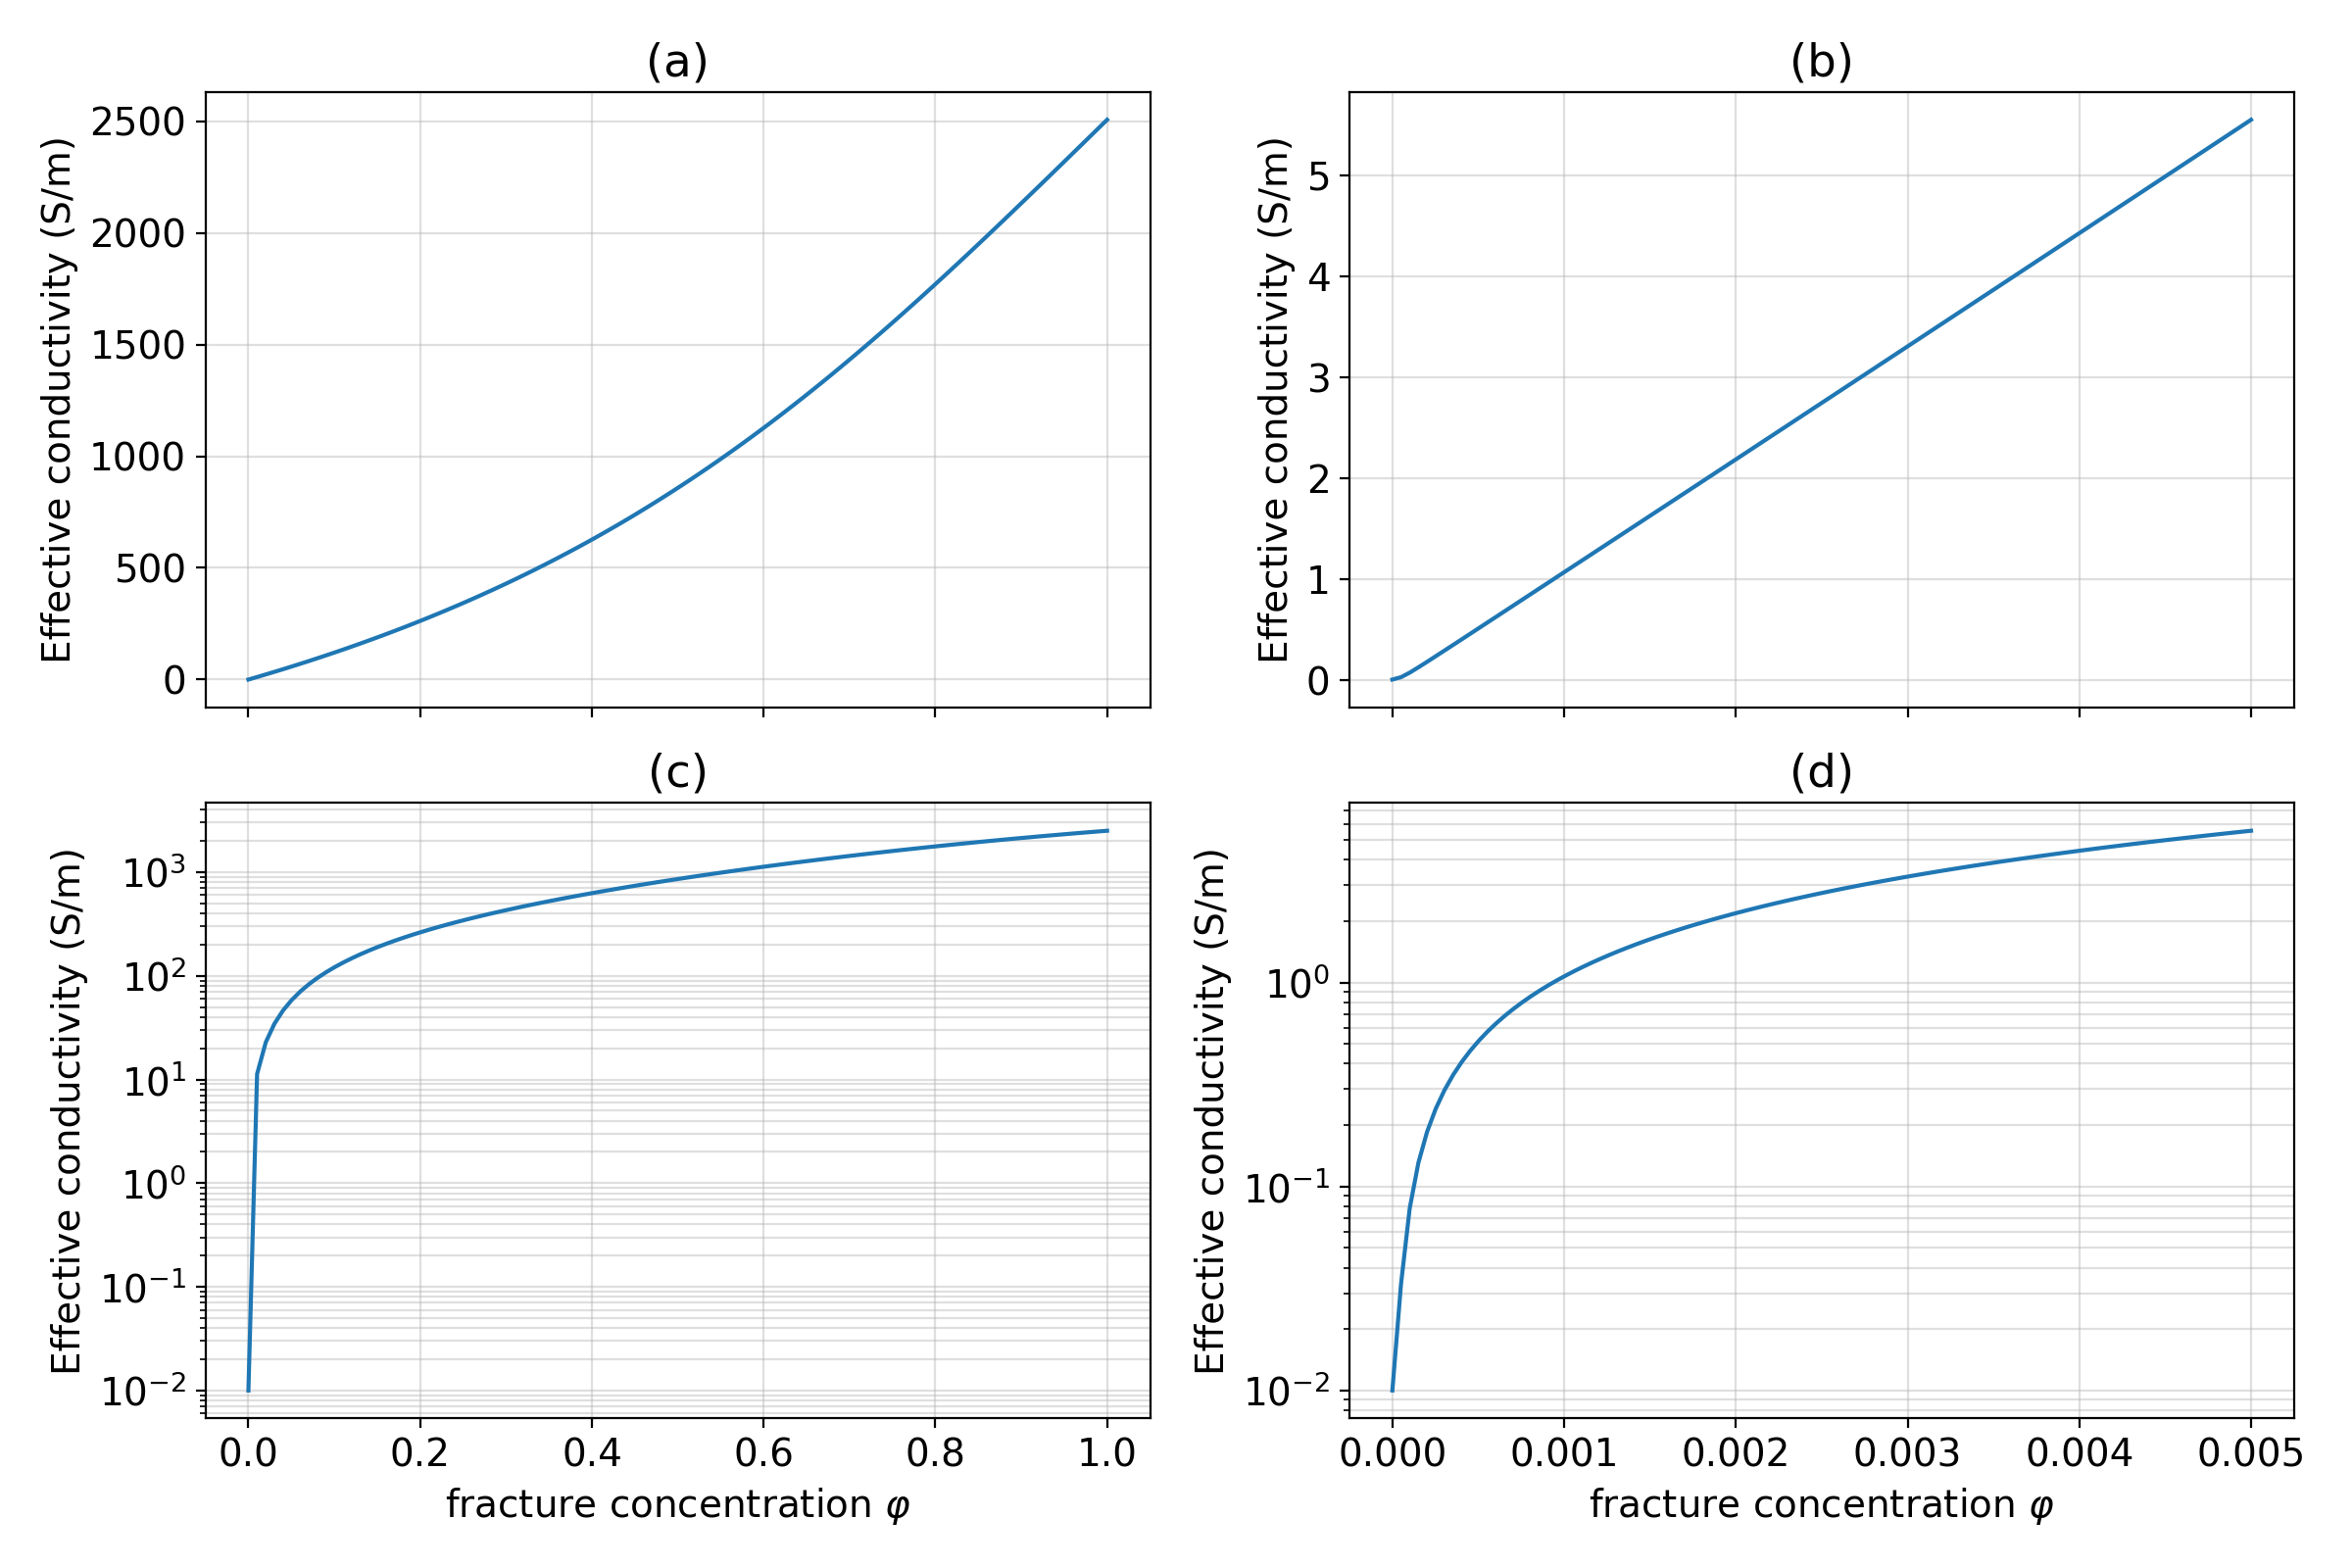
\includegraphics[width=0.8\textwidth]{figures/inversion/scemt_mapping.png}
    \end{center}
\caption{
   Self-consistent effective medium theory estimation of electrical conductivity as a function of fracture concentration.
   The conductivity of the background is $10^{-2}$ S/m and the conductivity of the material filling the fractures is 2500 S/m.
   We use an aspect ratio of $3 \times 10^{-5}$, and the fractures are assumed to be randomly oriented. Panels (a) and (b) show the
   conductivity on a linear scale while panels (c) and (d) show the conductivity on a logarithmic scale. Panels (a) and (c) show the
   full range of possible $\varphi$ values from 0 to 1, and panels (b) and (d) zoom into a smaller range, 0 $\leq \varphi \leq 0.005$.
}
\label{fig:scemt_mapping}
\end{figure}
